\documentclass{article}
\usepackage[T1]{fontenc}
\usepackage{lmodern}
\usepackage{graphicx}
\usepackage{amsmath,amssymb}
\usepackage[a4paper,margin=2cm]{geometry}
\usepackage[absolute,overlay]{textpos}
\setlength{\TPHorizModule}{1mm}
\setlength{\TPVertModule}{1mm}
\usepackage[indonesian]{babel}
\usepackage{hyperref}
\setlength{\emergencystretch}{2em}
% unit: Halaman 10

\begin{document}

% === Halaman 10 (llm) ===

\section*{Penjumlahan Titik pada Kurva Eliptik}

\vspace{190.08mm}

(a) $P + Q = R$

Penjelasan geometri:
\begin{enumerate}
  \item Tarik garis melalui $P$ dan $Q$
  \item Jika $P \neq Q$, garis tersebut memotong kurva pada titik $-R$
  \item Pencerminan titik $-R$ terhadap sumbu-x adalah titik $R$
  \item Titik $R$ adalah hasil penjumlahan titik $P$ dan $Q$
\end{enumerate}

\vspace{10mm}

Keterangan: Jika $R=(x, y)$ maka $-R$ adalah titik $(x, -y)$

\vspace{5mm}

\centering Sumber gambar: Andreas Steffen, Elliptic Curve Cryptography

% deskripsi: Grafik kurva eliptik yang mengilustrasikan geometri penjumlahan dua titik P dan Q untuk mendapatkan titik R, termasuk garis bantu dan titik -R sebagai hasil refleksi terhadap sumbu-x.
% bbox normalisasi: [0.4500, 0.2000, 0.8700, 0.8400]
\begin{textblock*}{88.20mm}(94.50mm,59.40mm)
\noindent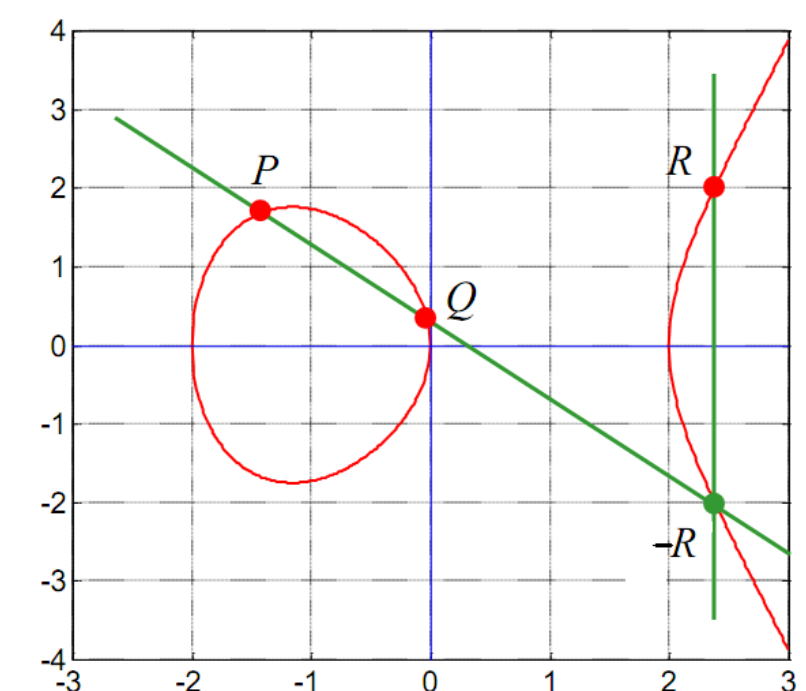
\includegraphics[width=88.20mm,height=190.08mm]{../../images/llm/page_010_img_01.png}%
\end{textblock*}

\end{document}
